\section{Vergleich}

% \begin{frame}{Vergleich der Invertierungsmethoden}
%     \begin{figure}
%         \centering
%         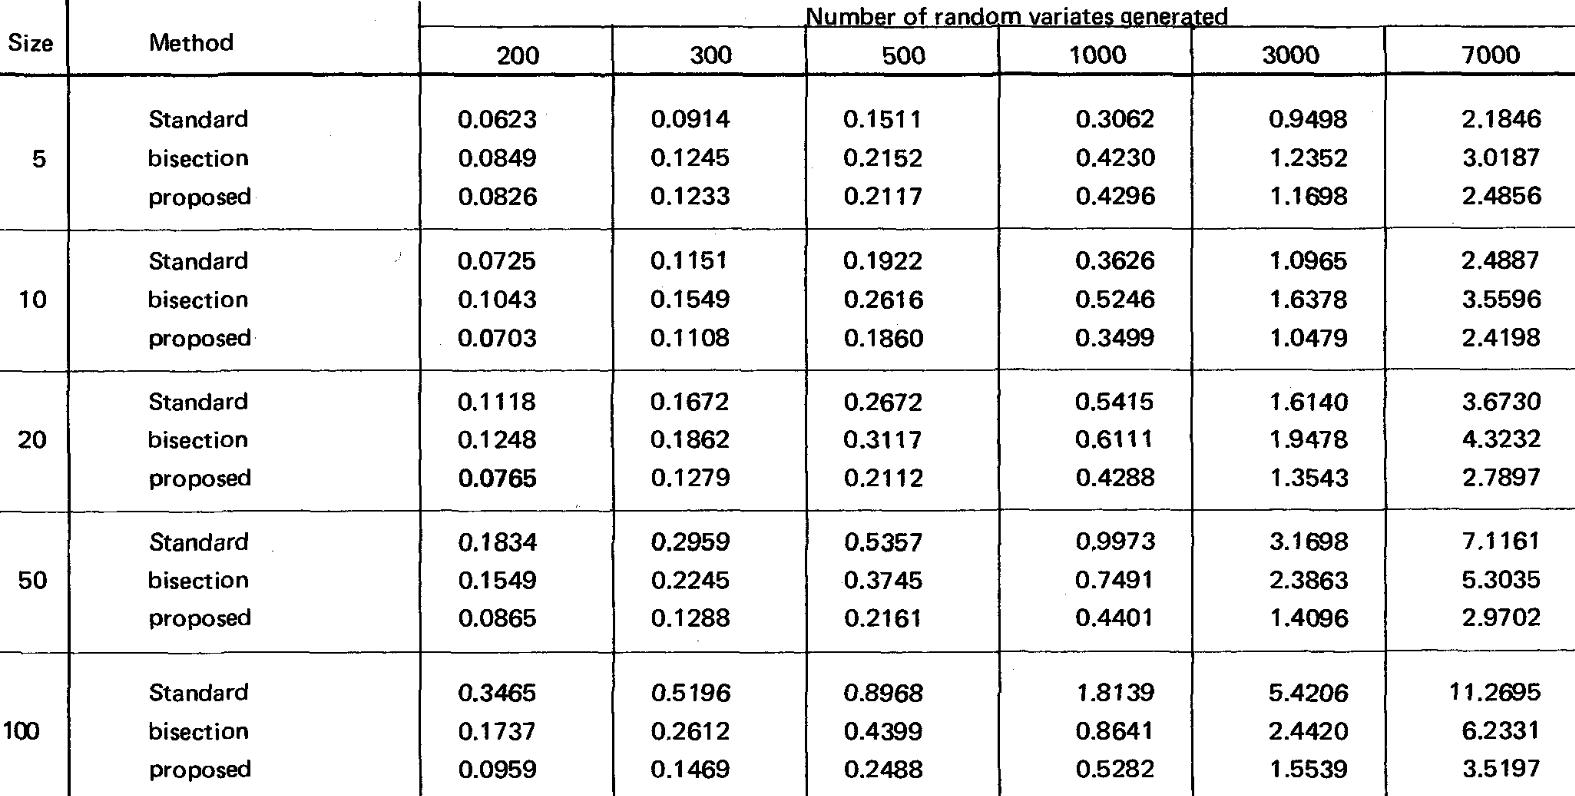
\includegraphics[width=.7\textwidth]{Screenshots/chenAsauHashTableComp.pdf}
%         \caption{\cite{chen_asau-generating_random_variates-1974}}
%     \end{figure}
% \end{frame}

\begin{frame}{Vergleich der Invertierungsmethoden}
    \begin{table}
        \centering
        \begin{tabular}{G|c|c|c|c|c|c|c}
            \rowcolor{Gray} &  & \multicolumn{6}{c}{Anzahl an generierten Zufallsvariablen} \\
            \cline{3-8}
            \rowcolor{Gray} \multirow{-2}{*}{Größe} & \multirow{-2}{*}{Methode} & 200 & 300 & 500 & 1000 & 3000 & 7000 \\
            \hline\hline
             & Standard & 0.0623\cellcolor<2-3>{pyblue} & 0.0914 & 0.1511 & 0.3062 & 0.9498 & 2.1846 \\
             & Binäre Suche & 0.08493\cellcolor<2-3>{pyblue} & 0.1245 & 0.2152 & 0.4230 & 1.2352 & 3.01873 \\
            \multirow{-3}{*}{5} & Hash-basiert & 0.0826\cellcolor<2-3>{pyorange} & 0.1233 & 0.2117 & 0.4296 & 1.1698 & 2.48563 \\
            \hline
            % \multirow{3}{*}{10} & Standard & 0.0123 & 0.0456 & 0.0789 & 0.1230 & 0.4567 & 0.8900 \\
            %  & Binäre Suche & 0.0123 & 0.0456 & 0.0789 & 0.1230 & 0.4567 & 0.8900 \\
            %  & Hash-basiert & 0.0123 & 0.0456 & 0.0789 & 0.1230 & 0.4567 & 0.8900 \\
            % \hline
            % \multirow{3}{*}{20} & Standard & 0.0123 & 0.0456 & 0.0789 & 0.1230 & 0.4567 & 0.8900 \\
            %  & Binäre Suche & 0.0123 & 0.0456 & 0.0789 & 0.1230 & 0.4567 & 0.8900 \\
            %  & Hash-basiert & 0.0123 & 0.0456 & 0.0789 & 0.1230 & 0.4567 & 0.8900 \\
            % \hline
             & Standard & 0.1834 & 0.2959 & 0.5357 & 0.9973 & 3.1 698 & 7.1161 \\
             & Binäre Suche &  0.1549 & 0.2245 & 0.3745 & 0.7491 & 2.3863 & 5.3035 \\
            \multirow{-3}{*}{50} & Hash-basiert & 0.0865 & 0.1288 & 0.2161 & 0.4401 & 1.4096 & 2.970 \\
            \hline
             & Standard & 0.3465 & 0.5 196 & 0.8968 & 1.8139 & 5.4206 & 11.2695\cellcolor<3>{pyblue} \\
             & Binäre Suche & 0.17373 & 0.261 2 & 0.4399 & 0.8641 & 2.4420 & 6.23313\cellcolor<3>{pyblue} \\
            \multirow{-3}{*}{100} & Hash-basiert & 0.09593 & 0.1 469 & 0.2488 & 0.5282 & 1.5539 & 3.51973\cellcolor<3>{pyorange}
        \end{tabular}
        \caption{\cite{chen_asau-generating_random_variates-1974}}
    \end{table}
\end{frame}

